\documentclass{standalone}
\usepackage{tikz}
\usepackage{ctex,siunitx}
\setCJKmainfont{Noto Serif CJK SC}
\usepackage{tkz-euclide}
\usepackage{amsmath}
\usetikzlibrary{patterns, calc}
\usetikzlibrary {decorations.pathmorphing, decorations.pathreplacing, decorations.shapes,}

\begin{document}
\small
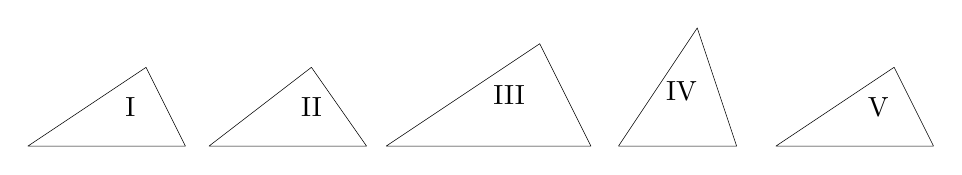
\begin{tikzpicture}[>=stealth,scale=1]
  \tkzSetUpPoint[fill=black]
  % \useasboundingbox(-1,-0.75)rectangle(3.7,1.4);
  \begin{scope}
  \tkzDefPoints{0/0/A, 2/0/B, 1.5/1/C}
  \tkzDrawPolygon(A,B,C)
  \node at (1.3,.5){I};
  \end{scope}
  \begin{scope}[xshift=2.3cm]
    \tkzDefPoints{0/0/A, 2/0/B, 1.3/1/C}
  \tkzDrawPolygon(A,B,C)
  \node at (1.3,.5){II};
  \end{scope}
  \begin{scope}[scale=1.3, xshift=3.5cm]
    \tkzDefPoints{0/0/A, 2/0/B, 1.5/1/C}
  \tkzDrawPolygon(A,B,C)
  \node at (1.2,.5){III};
  \end{scope}
  \begin{scope}[xshift=7.5cm]
    \tkzDefPoints{0/0/A, 1.5/0/B, 1/1.5/C}
  \tkzDrawPolygon(A,B,C)
  \node at (.8,.7){IV};
  \end{scope}
  \begin{scope}[xshift=9.5cm]
    \tkzDefPoints{0/0/A, 2/0/B, 1.5/1/C}
  \tkzDrawPolygon(A,B,C)
  \node at (1.3,.5){V};
  \end{scope}
\end{tikzpicture}
\end{document}